\section{Introduction}
\label{sec:introduction}

\begin{figure}[t]
\centering
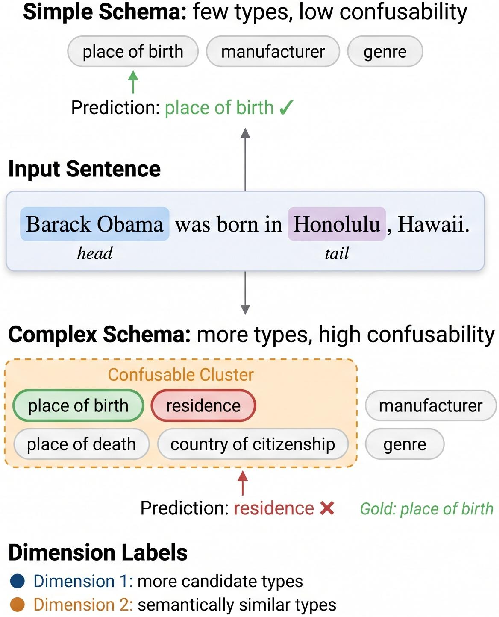
\includegraphics[width=\columnwidth]{../../figures/paper/fig_problem_illustration.pdf}
\caption{Schema complexity in zero-shot relation extraction. Given the same input, a simple schema (few dissimilar types) yields the correct relation, while a complex schema with more candidate types and a cluster of semantically similar types causes type substitution (gold \emph{place of birth} $\to$ predicted \emph{residence}). We decompose schema complexity into two dimensions: type count and inter-type confusability.}
\label{fig:problem}
\end{figure}

\looseness=-1
Training-free\footnote{We use ``training-free'' and ``zero-shot'' interchangeably to denote prompting without parameter updates.} LLM information extraction (prompting a large language model with a target schema and asking it to extract structured information without any task-specific fine-tuning) enables rapid deployment across new domains and ontologies. This zero-shot paradigm eliminates the need for labeled data, and is attractive for applications where annotation is expensive or schemas evolve frequently \citep{llm4ie-survey-2024}. Yet the paradigm carries a critical limitation: performance degrades sharply as the number of candidate types in the prompt schema grows. On named entity recognition, recall drops from 0.72 with a single candidate type to a plateau of ${\sim}$0.28 across intermediate schema sizes (22--44 types) before partial recovery at full-schema. On relation extraction, accuracy falls from 85.7\% with one relation to 50.4\% with 80 relations (sentence-level) and from 88.0\% to 38.7\% with 96 relations (document-level), near-halving or worse. This degradation is not academic: real-world ontologies routinely define 50--200+ types, which places them squarely in the regime where training-free extraction becomes unreliable (Figure~\ref{fig:problem}).

\looseness=-1
What explains this degradation? Prior decomposition strategies \citep{uniner-2024,llm-pee-2025,parse-2025} conflate two factors: having more types to discriminate among (count) and having semantically similar types to confuse (confusability) (hereafter Dimension~1 and Dimension~2). None isolates which factor predicts the gains (\S\ref{sec:related_work}).

This study combines correlational analyses with quasi-experimental manipulation (confusability-controlled batches) to characterize how schema properties predict extraction accuracy (Figure~\ref{fig:framework}).

We ask three questions. \textbf{RQ1}: Does type confusability independently predict extraction degradation beyond the effect of type count? \textbf{RQ2}: Through what modes do count and confusability each degrade performance? \textbf{RQ3}: Can confusability-aware schema decomposition improve extraction quality?

\looseness=-1
To our knowledge, we present the first controlled study simultaneously isolating type count and inter-type confusability as independent dimensions via embedding-based metrics and stratified batch design in zero-shot LLM IE, spanning NER, RE, and event detection (ED). We quantify confusability using pairwise embedding similarity, the \emph{Schema Confusability Score} (SCS), and its batch-level aggregation, the \emph{Batch Confusability Score} (BCS). We evaluate on Few-NERD \citep{fewnerd-2021}, FewRel \citep{fewrel-2018}, DocRED \citep{docred-2019}, and MAVEN \citep{maven-2020} using Qwen3-32B (\S\ref{sec:experimental_setup}).

Our contributions are:
\begin{enumerate}[leftmargin=*,itemsep=2pt,topsep=2pt]
    \item We find that type confusability, quantified by embedding similarity (SCS/BCS, building on \citealt{llm-pee-2025}), independently predicts type substitution errors in RE on FewRel (variance inflation factor [VIF]${}\,=\,1.18$), independently explaining ${\sim}$27\% of batch-level variance (semipartial $R^2 = 0.273$; ecological level). This finding is enabled by BCS-controlled batch design that isolates confusability from type count, a methodology not previously applied in training-free LLM IE (\S\ref{sec:count_curves}, \S\ref{sec:pairwise}, \S\ref{sec:bcs_controlled}).
    \item We document a task-dependent boundary: the RE confusability effect is replicated across two model families (three scales), with no detected format dependence, while the NER batch-level BCS null (reported as a boundary condition rather than a negative result) is attributable to dispersed error modes (miss, boundary, type) and BCS range compression (\S\ref{sec:bcs_controlled}, \S\ref{sec:multi_channel}).
    \item We identify structural barriers to confusability-aware extraction: schema decomposition fails due to merge amplification (NER, ED) and routing failure (RE). The decompose-then-merge paradigm faces structural precision--recall tradeoffs in training-free IE (\S\ref{sec:sdgd}).
\end{enumerate}

% Figure 2 (fig:framework) moved to related_work.tex for page distribution